% Figure 1: headline result at a glance, two regimes side by side.
% Deliberately plain TikZ (no pgfplots) -- manual rectangles/lines only,
% to minimize the risk of a library-version compile failure. Values are
% Qwen2.5-7B-Instruct, n=100, from Table~\ref{tab:no_relay}.
%
% RISK NOTE: this file was written without the ability to compile it.
% Check it renders correctly in Overleaf before relying on it -- if it
% fails to compile, comment out the % Figure 1: headline result at a glance, two regimes side by side.
% Deliberately plain TikZ (no pgfplots) -- manual rectangles/lines only,
% to minimize the risk of a library-version compile failure. Values are
% Qwen2.5-7B-Instruct, n=100, from Table~\ref{tab:no_relay}.
%
% RISK NOTE: this file was written without the ability to compile it.
% Check it renders correctly in Overleaf before relying on it -- if it
% fails to compile, comment out the % Figure 1: headline result at a glance, two regimes side by side.
% Deliberately plain TikZ (no pgfplots) -- manual rectangles/lines only,
% to minimize the risk of a library-version compile failure. Values are
% Qwen2.5-7B-Instruct, n=100, from Table~\ref{tab:no_relay}.
%
% RISK NOTE: this file was written without the ability to compile it.
% Check it renders correctly in Overleaf before relying on it -- if it
% fails to compile, comment out the % Figure 1: headline result at a glance, two regimes side by side.
% Deliberately plain TikZ (no pgfplots) -- manual rectangles/lines only,
% to minimize the risk of a library-version compile failure. Values are
% Qwen2.5-7B-Instruct, n=100, from Table~\ref{tab:no_relay}.
%
% RISK NOTE: this file was written without the ability to compile it.
% Check it renders correctly in Overleaf before relying on it -- if it
% fails to compile, comment out the \input{figure1_overview} line in
% main_v5.tex (the rest of the paper does not depend on this figure) and
% report the exact error back.

\begin{figure*}[t]
\centering
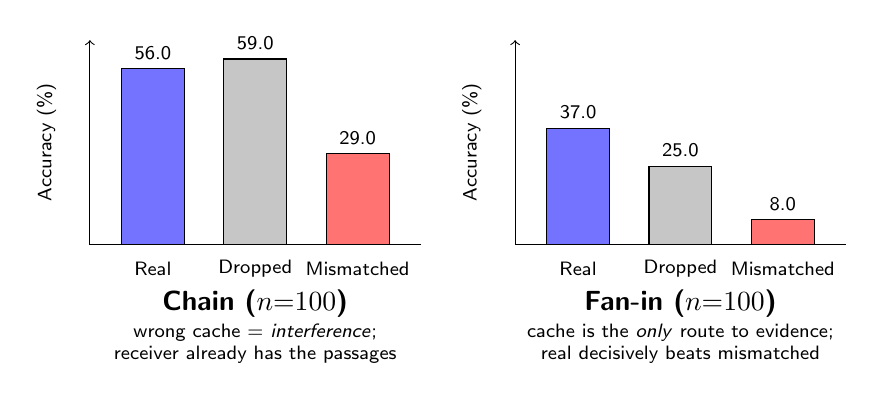
\begin{tikzpicture}[x=1cm, y=1cm, every node/.style={font=\sffamily}]

% ---------- Panel 1: Chain ----------
\begin{scope}[xshift=0cm]
  % axis
  \draw[->] (0,0) -- (0,2.6);
  \draw (0,0) -- (4.2,0);
  \node[rotate=90, font=\sffamily\scriptsize] at (-0.55,1.3) {Accuracy (\%)};

  % bar: Real = 56.0
  \draw[fill=blue!55] (0.4,0) rectangle (1.2,2.24);
  \node[font=\sffamily\scriptsize] at (0.8,2.44) {56.0};
  \node[font=\sffamily\scriptsize] at (0.8,-0.3) {Real};

  % bar: Dropped = 59.0
  \draw[fill=gray!45] (1.7,0) rectangle (2.5,2.36);
  \node[font=\sffamily\scriptsize] at (2.1,2.56) {59.0};
  \node[font=\sffamily\scriptsize] at (2.1,-0.3) {Dropped};

  % bar: Mismatched = 29.0
  \draw[fill=red!55] (3.0,0) rectangle (3.8,1.16);
  \node[font=\sffamily\scriptsize] at (3.4,1.36) {29.0};
  \node[font=\sffamily\scriptsize] at (3.4,-0.3) {Mismatched};

  \node[font=\sffamily\bfseries] at (2.1,-0.75) {Chain ($n{=}100$)};
  \node[font=\sffamily\scriptsize, align=center] at (2.1,-1.25)
    {wrong cache = \textit{interference};\\receiver already has the passages};
\end{scope}

% ---------- Panel 2: Fan-in ----------
\begin{scope}[xshift=5.4cm]
  \draw[->] (0,0) -- (0,2.6);
  \draw (0,0) -- (4.2,0);
  \node[rotate=90, font=\sffamily\scriptsize] at (-0.55,1.3) {Accuracy (\%)};

  % bar: Real = 37.0
  \draw[fill=blue!55] (0.4,0) rectangle (1.2,1.48);
  \node[font=\sffamily\scriptsize] at (0.8,1.68) {37.0};
  \node[font=\sffamily\scriptsize] at (0.8,-0.3) {Real};

  % bar: Dropped = 25.0
  \draw[fill=gray!45] (1.7,0) rectangle (2.5,1.00);
  \node[font=\sffamily\scriptsize] at (2.1,1.20) {25.0};
  \node[font=\sffamily\scriptsize] at (2.1,-0.3) {Dropped};

  % bar: Mismatched = 8.0
  \draw[fill=red!55] (3.0,0) rectangle (3.8,0.32);
  \node[font=\sffamily\scriptsize] at (3.4,0.52) {8.0};
  \node[font=\sffamily\scriptsize] at (3.4,-0.3) {Mismatched};

  \node[font=\sffamily\bfseries] at (2.1,-0.75) {Fan-in ($n{=}100$)};
  \node[font=\sffamily\scriptsize, align=center] at (2.1,-1.25)
    {cache is the \textit{only} route to evidence;\\real decisively beats mismatched};
\end{scope}

\end{tikzpicture}
\caption{\textbf{Takeaway: a wrong cache is worse than no cache at all
in both topologies we test (Qwen2.5-7B-Instruct, $n{=}100$), but
whether the \emph{correct} cache beats no cache depends entirely on
whether the receiver has another way to get the same information.} In
the chain (left), the receiver's own prompt already contains the source
passages, so dropped ($59.0\%$) is statistically indistinguishable from
real ($56.0\%$, $p=0.68$) -- but mismatched ($29.0\%$) is far worse than
either ($p<0.0001$ vs.\ both). In the fan-in (right), the aggregator has
no independent copy of the passages, so real ($37.0\%$) decisively
beats mismatched ($8.0\%$, $p<0.0001$), and even the real-vs-dropped gap
trends toward significance ($p=0.050$) rather than away from it. Full
statistics, all three models, and the dropped-vs-mismatched legs in
Table~\ref{tab:no_relay}.}
\label{fig:headline}
\end{figure*}
 line in
% main_v5.tex (the rest of the paper does not depend on this figure) and
% report the exact error back.

\begin{figure*}[t]
\centering
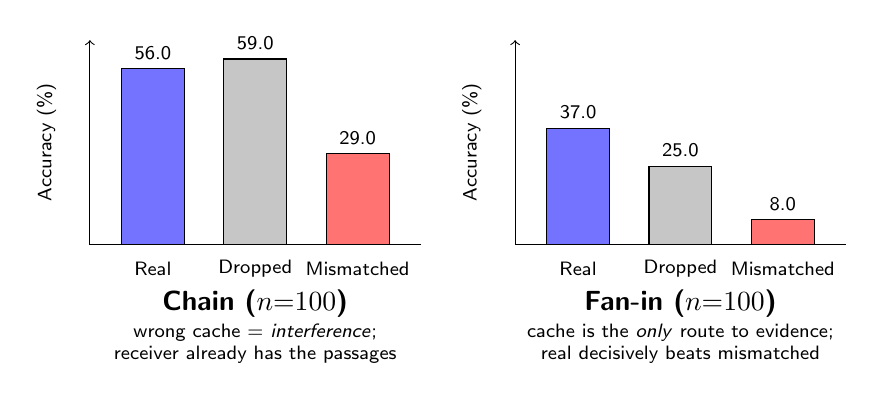
\begin{tikzpicture}[x=1cm, y=1cm, every node/.style={font=\sffamily}]

% ---------- Panel 1: Chain ----------
\begin{scope}[xshift=0cm]
  % axis
  \draw[->] (0,0) -- (0,2.6);
  \draw (0,0) -- (4.2,0);
  \node[rotate=90, font=\sffamily\scriptsize] at (-0.55,1.3) {Accuracy (\%)};

  % bar: Real = 56.0
  \draw[fill=blue!55] (0.4,0) rectangle (1.2,2.24);
  \node[font=\sffamily\scriptsize] at (0.8,2.44) {56.0};
  \node[font=\sffamily\scriptsize] at (0.8,-0.3) {Real};

  % bar: Dropped = 59.0
  \draw[fill=gray!45] (1.7,0) rectangle (2.5,2.36);
  \node[font=\sffamily\scriptsize] at (2.1,2.56) {59.0};
  \node[font=\sffamily\scriptsize] at (2.1,-0.3) {Dropped};

  % bar: Mismatched = 29.0
  \draw[fill=red!55] (3.0,0) rectangle (3.8,1.16);
  \node[font=\sffamily\scriptsize] at (3.4,1.36) {29.0};
  \node[font=\sffamily\scriptsize] at (3.4,-0.3) {Mismatched};

  \node[font=\sffamily\bfseries] at (2.1,-0.75) {Chain ($n{=}100$)};
  \node[font=\sffamily\scriptsize, align=center] at (2.1,-1.25)
    {wrong cache = \textit{interference};\\receiver already has the passages};
\end{scope}

% ---------- Panel 2: Fan-in ----------
\begin{scope}[xshift=5.4cm]
  \draw[->] (0,0) -- (0,2.6);
  \draw (0,0) -- (4.2,0);
  \node[rotate=90, font=\sffamily\scriptsize] at (-0.55,1.3) {Accuracy (\%)};

  % bar: Real = 37.0
  \draw[fill=blue!55] (0.4,0) rectangle (1.2,1.48);
  \node[font=\sffamily\scriptsize] at (0.8,1.68) {37.0};
  \node[font=\sffamily\scriptsize] at (0.8,-0.3) {Real};

  % bar: Dropped = 25.0
  \draw[fill=gray!45] (1.7,0) rectangle (2.5,1.00);
  \node[font=\sffamily\scriptsize] at (2.1,1.20) {25.0};
  \node[font=\sffamily\scriptsize] at (2.1,-0.3) {Dropped};

  % bar: Mismatched = 8.0
  \draw[fill=red!55] (3.0,0) rectangle (3.8,0.32);
  \node[font=\sffamily\scriptsize] at (3.4,0.52) {8.0};
  \node[font=\sffamily\scriptsize] at (3.4,-0.3) {Mismatched};

  \node[font=\sffamily\bfseries] at (2.1,-0.75) {Fan-in ($n{=}100$)};
  \node[font=\sffamily\scriptsize, align=center] at (2.1,-1.25)
    {cache is the \textit{only} route to evidence;\\real decisively beats mismatched};
\end{scope}

\end{tikzpicture}
\caption{\textbf{Takeaway: a wrong cache is worse than no cache at all
in both topologies we test (Qwen2.5-7B-Instruct, $n{=}100$), but
whether the \emph{correct} cache beats no cache depends entirely on
whether the receiver has another way to get the same information.} In
the chain (left), the receiver's own prompt already contains the source
passages, so dropped ($59.0\%$) is statistically indistinguishable from
real ($56.0\%$, $p=0.68$) -- but mismatched ($29.0\%$) is far worse than
either ($p<0.0001$ vs.\ both). In the fan-in (right), the aggregator has
no independent copy of the passages, so real ($37.0\%$) decisively
beats mismatched ($8.0\%$, $p<0.0001$), and even the real-vs-dropped gap
trends toward significance ($p=0.050$) rather than away from it. Full
statistics, all three models, and the dropped-vs-mismatched legs in
Table~\ref{tab:no_relay}.}
\label{fig:headline}
\end{figure*}
 line in
% main_v5.tex (the rest of the paper does not depend on this figure) and
% report the exact error back.

\begin{figure*}[t]
\centering
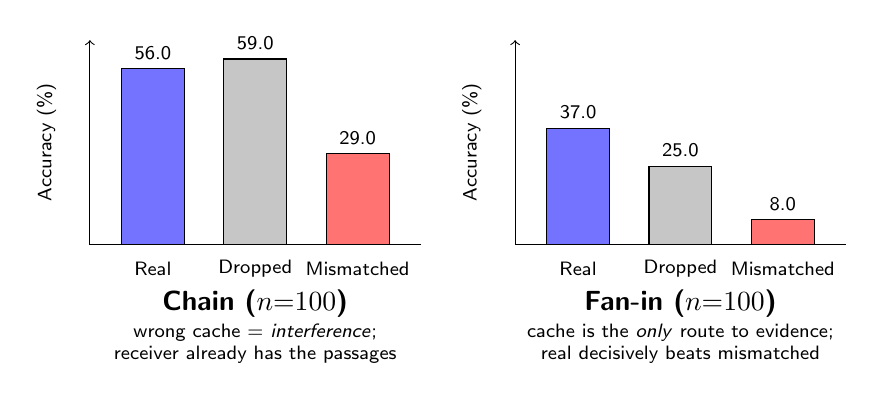
\begin{tikzpicture}[x=1cm, y=1cm, every node/.style={font=\sffamily}]

% ---------- Panel 1: Chain ----------
\begin{scope}[xshift=0cm]
  % axis
  \draw[->] (0,0) -- (0,2.6);
  \draw (0,0) -- (4.2,0);
  \node[rotate=90, font=\sffamily\scriptsize] at (-0.55,1.3) {Accuracy (\%)};

  % bar: Real = 56.0
  \draw[fill=blue!55] (0.4,0) rectangle (1.2,2.24);
  \node[font=\sffamily\scriptsize] at (0.8,2.44) {56.0};
  \node[font=\sffamily\scriptsize] at (0.8,-0.3) {Real};

  % bar: Dropped = 59.0
  \draw[fill=gray!45] (1.7,0) rectangle (2.5,2.36);
  \node[font=\sffamily\scriptsize] at (2.1,2.56) {59.0};
  \node[font=\sffamily\scriptsize] at (2.1,-0.3) {Dropped};

  % bar: Mismatched = 29.0
  \draw[fill=red!55] (3.0,0) rectangle (3.8,1.16);
  \node[font=\sffamily\scriptsize] at (3.4,1.36) {29.0};
  \node[font=\sffamily\scriptsize] at (3.4,-0.3) {Mismatched};

  \node[font=\sffamily\bfseries] at (2.1,-0.75) {Chain ($n{=}100$)};
  \node[font=\sffamily\scriptsize, align=center] at (2.1,-1.25)
    {wrong cache = \textit{interference};\\receiver already has the passages};
\end{scope}

% ---------- Panel 2: Fan-in ----------
\begin{scope}[xshift=5.4cm]
  \draw[->] (0,0) -- (0,2.6);
  \draw (0,0) -- (4.2,0);
  \node[rotate=90, font=\sffamily\scriptsize] at (-0.55,1.3) {Accuracy (\%)};

  % bar: Real = 37.0
  \draw[fill=blue!55] (0.4,0) rectangle (1.2,1.48);
  \node[font=\sffamily\scriptsize] at (0.8,1.68) {37.0};
  \node[font=\sffamily\scriptsize] at (0.8,-0.3) {Real};

  % bar: Dropped = 25.0
  \draw[fill=gray!45] (1.7,0) rectangle (2.5,1.00);
  \node[font=\sffamily\scriptsize] at (2.1,1.20) {25.0};
  \node[font=\sffamily\scriptsize] at (2.1,-0.3) {Dropped};

  % bar: Mismatched = 8.0
  \draw[fill=red!55] (3.0,0) rectangle (3.8,0.32);
  \node[font=\sffamily\scriptsize] at (3.4,0.52) {8.0};
  \node[font=\sffamily\scriptsize] at (3.4,-0.3) {Mismatched};

  \node[font=\sffamily\bfseries] at (2.1,-0.75) {Fan-in ($n{=}100$)};
  \node[font=\sffamily\scriptsize, align=center] at (2.1,-1.25)
    {cache is the \textit{only} route to evidence;\\real decisively beats mismatched};
\end{scope}

\end{tikzpicture}
\caption{\textbf{Takeaway: a wrong cache is worse than no cache at all
in both topologies we test (Qwen2.5-7B-Instruct, $n{=}100$), but
whether the \emph{correct} cache beats no cache depends entirely on
whether the receiver has another way to get the same information.} In
the chain (left), the receiver's own prompt already contains the source
passages, so dropped ($59.0\%$) is statistically indistinguishable from
real ($56.0\%$, $p=0.68$) -- but mismatched ($29.0\%$) is far worse than
either ($p<0.0001$ vs.\ both). In the fan-in (right), the aggregator has
no independent copy of the passages, so real ($37.0\%$) decisively
beats mismatched ($8.0\%$, $p<0.0001$), and even the real-vs-dropped gap
trends toward significance ($p=0.050$) rather than away from it. Full
statistics, all three models, and the dropped-vs-mismatched legs in
Table~\ref{tab:no_relay}.}
\label{fig:headline}
\end{figure*}
 line in
% main_v5.tex (the rest of the paper does not depend on this figure) and
% report the exact error back.

\begin{figure*}[t]
\centering
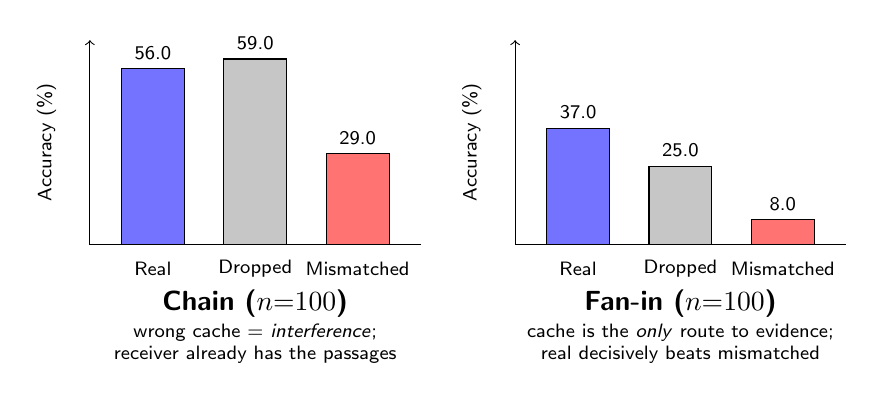
\begin{tikzpicture}[x=1cm, y=1cm, every node/.style={font=\sffamily}]

% ---------- Panel 1: Chain ----------
\begin{scope}[xshift=0cm]
  % axis
  \draw[->] (0,0) -- (0,2.6);
  \draw (0,0) -- (4.2,0);
  \node[rotate=90, font=\sffamily\scriptsize] at (-0.55,1.3) {Accuracy (\%)};

  % bar: Real = 56.0
  \draw[fill=blue!55] (0.4,0) rectangle (1.2,2.24);
  \node[font=\sffamily\scriptsize] at (0.8,2.44) {56.0};
  \node[font=\sffamily\scriptsize] at (0.8,-0.3) {Real};

  % bar: Dropped = 59.0
  \draw[fill=gray!45] (1.7,0) rectangle (2.5,2.36);
  \node[font=\sffamily\scriptsize] at (2.1,2.56) {59.0};
  \node[font=\sffamily\scriptsize] at (2.1,-0.3) {Dropped};

  % bar: Mismatched = 29.0
  \draw[fill=red!55] (3.0,0) rectangle (3.8,1.16);
  \node[font=\sffamily\scriptsize] at (3.4,1.36) {29.0};
  \node[font=\sffamily\scriptsize] at (3.4,-0.3) {Mismatched};

  \node[font=\sffamily\bfseries] at (2.1,-0.75) {Chain ($n{=}100$)};
  \node[font=\sffamily\scriptsize, align=center] at (2.1,-1.25)
    {wrong cache = \textit{interference};\\receiver already has the passages};
\end{scope}

% ---------- Panel 2: Fan-in ----------
\begin{scope}[xshift=5.4cm]
  \draw[->] (0,0) -- (0,2.6);
  \draw (0,0) -- (4.2,0);
  \node[rotate=90, font=\sffamily\scriptsize] at (-0.55,1.3) {Accuracy (\%)};

  % bar: Real = 37.0
  \draw[fill=blue!55] (0.4,0) rectangle (1.2,1.48);
  \node[font=\sffamily\scriptsize] at (0.8,1.68) {37.0};
  \node[font=\sffamily\scriptsize] at (0.8,-0.3) {Real};

  % bar: Dropped = 25.0
  \draw[fill=gray!45] (1.7,0) rectangle (2.5,1.00);
  \node[font=\sffamily\scriptsize] at (2.1,1.20) {25.0};
  \node[font=\sffamily\scriptsize] at (2.1,-0.3) {Dropped};

  % bar: Mismatched = 8.0
  \draw[fill=red!55] (3.0,0) rectangle (3.8,0.32);
  \node[font=\sffamily\scriptsize] at (3.4,0.52) {8.0};
  \node[font=\sffamily\scriptsize] at (3.4,-0.3) {Mismatched};

  \node[font=\sffamily\bfseries] at (2.1,-0.75) {Fan-in ($n{=}100$)};
  \node[font=\sffamily\scriptsize, align=center] at (2.1,-1.25)
    {cache is the \textit{only} route to evidence;\\real decisively beats mismatched};
\end{scope}

\end{tikzpicture}
\caption{\textbf{Takeaway: a wrong cache is worse than no cache at all
in both topologies we test (Qwen2.5-7B-Instruct, $n{=}100$), but
whether the \emph{correct} cache beats no cache depends entirely on
whether the receiver has another way to get the same information.} In
the chain (left), the receiver's own prompt already contains the source
passages, so dropped ($59.0\%$) is statistically indistinguishable from
real ($56.0\%$, $p=0.68$) -- but mismatched ($29.0\%$) is far worse than
either ($p<0.0001$ vs.\ both). In the fan-in (right), the aggregator has
no independent copy of the passages, so real ($37.0\%$) decisively
beats mismatched ($8.0\%$, $p<0.0001$), and even the real-vs-dropped gap
trends toward significance ($p=0.050$) rather than away from it. Full
statistics, all three models, and the dropped-vs-mismatched legs in
Table~\ref{tab:no_relay}.}
\label{fig:headline}
\end{figure*}
